\documentclass{beamer}
\usepackage[utf8]{inputenc}

\usetheme{Madrid}
\usecolortheme{default}
\usepackage{amsmath,amssymb,amsfonts,amsthm}
\usepackage{txfonts}
\usepackage{tkz-euclide}
\usepackage{listings}
\usepackage{adjustbox}
\usepackage{array}
\usepackage{tabularx}
\usepackage{gvv}
\usepackage{lmodern}
\usepackage{circuitikz}
\usepackage{tikz}
\usepackage{graphicx}

\setbeamertemplate{page number in head/foot}[totalframenumber]

\usepackage{tcolorbox}
\tcbuselibrary{minted,breakable,xparse,skins}



\definecolor{bg}{gray}{0.95}
\DeclareTCBListing{mintedbox}{O{}m!O{}}{%
  breakable=true,
  listing engine=minted,
  listing only,
  minted language=#2,
  minted style=default,
  minted options={%
    linenos,
    gobble=0,
    breaklines=true,
    breakafter=,,
    fontsize=\small,
    numbersep=8pt,
    #1},
  boxsep=0pt,
  left skip=0pt,
  right skip=0pt,
  left=25pt,
  right=0pt,
  top=3pt,
  bottom=3pt,
  arc=5pt,
  leftrule=0pt,
  rightrule=0pt,
  bottomrule=2pt,
  toprule=2pt,
  colback=bg,
  colframe=orange!70,
  enhanced,
  overlay={%
    \begin{tcbclipinterior}
    \fill[orange!20!white] (frame.south west) rectangle ([xshift=20pt]frame.north west);
    \end{tcbclipinterior}},
  #3,
}
\lstset{
    language=C,
    basicstyle=\ttfamily\small,
    keywordstyle=\color{blue},
    stringstyle=\color{orange},
    commentstyle=\color{green!60!black},
    numbers=left,
    numberstyle=\tiny\color{gray},
    breaklines=true,
    showstringspaces=false,
}
%------------------------------------------------------------
%This block of code defines the information to appear in the
%Title page
\title %optional
{1.9.18}
\date{August 31,2025}


\author 
{Jnanesh Sathisha karmar - EE25BTECH11029}



\begin{document}



\frame{\titlepage}
\begin{frame}{Question}
Find the value of $x$ if the distance between the points $\vec{A}\brak{0, 0}$ and $\vec{B}\brak{x, -4}$ is $5$ units.
\end{frame}



\begin{frame}{Equation}

Distance between 2 vectors $\vec{A}$ and $\vec{B}$ can be represented as:
\begin{align}
    \norm{AB}=\sqrt{\brak{\vec{B}-\vec{A}}^T\brak{\vec{B}-\vec{A}}}
\end{align}
\end{frame}

\begin{frame}{Theoretical Solution}

Given details:
\begin{align}
    \vec{A}=\myvec{0\\0}\\  \vec{B}=\myvec{x\\-4}\\ \norm{AB}=5 
\end{align}
\end{frame}

\begin{frame}{Theoretical Solution}

By substituting values:
\begin{align}
    \norm{AB}=\sqrt{\myvec{x & -4}\myvec{x \\-4}}=\sqrt{x^2 + \brak{-4}^2}=\sqrt{x^2+16}
\end{align}

\end{frame}


\begin{frame}{Theoretical Solution}
Now comparing it with the given distance:
\begin{align}
    \sqrt{x^2+16}=5
\end{align}
Square on both sides
\begin{align}
    x^2 +16=25\\
    x^2=9\\
    x=3\  or\ x=-3 
\end{align}

\end{frame}
\begin{frame}{Theoretical Solution}
\textbf{Final answer:}\\
The values of $x$ are $3$ and $-3$
\end{frame}

\begin{frame}[fragile]
    \frametitle{C Code (1) - Function to generate a line segment }

    \begin{lstlisting}

#include <math.h>

// Function to calculate distance between two points (x1,y1) and (x2,y2)
double distance(double x1, double y1, double x2, double y2) {
    double dx = x2 - x1;
    double dy = y2 - y1;
    return sqrt(dx * dx + dy * dy);
}

    \end{lstlisting}
\end{frame}


\begin{frame}[fragile]
    \frametitle{Python Code - Using Shared Object}
    \begin{lstlisting}

import ctypes
import numpy as np
import matplotlib.pyplot as plt

# Load shared object
lib = ctypes.CDLL("./libline.so")

# Define function signature
lib.distance.argtypes = [ctypes.c_double, ctypes.c_double,
                         ctypes.c_double, ctypes.c_double]
lib.distance.restype = ctypes.c_double


   



\end{lstlisting}
\end{frame}

\begin{frame}[fragile]
    \frametitle{Python Code - Using Shared Object}
    \begin{lstlisting}
# Fixed point A
A = (0, 0)

# Two B points
B1 = (3, -4)
B2 = (-3, 4)

# Distances from A using C function
d1 = lib.distance(A[0], A[1], B1[0], B1[1])
d2 = lib.distance(A[0], A[1], B2[0], B2[1])

# Plot line segments A->B1 and A->B2
plt.figure(figsize=(6,6))

\end{lstlisting}
\end{frame}
\begin{frame}[fragile]
    \frametitle{Python Code - Using Shared Object}
    \begin{lstlisting}
# Line A->B1
plt.plot([A[0], B1[0]], [A[1], B1[1]], 'b-o', label=f"A→B1 {B1}, d={d1:.2f}")
plt.text(B1[0], B1[1], f"B1{B1}", fontsize=12, ha='left')

# Line A->B2
plt.plot([A[0], B2[0]], [A[1], B2[1]], 'g-o', label=f"A→B2 {B2}, d={d2:.2f}")
plt.text(B2[0], B2[1], f"B2{B2}", fontsize=12, ha='left')

# Mark A
plt.scatter(A[0], A[1], color='red')
plt.text(A[0], A[1], "A(0,0)", fontsize=12, ha='right')




\end{lstlisting}
\end{frame}
\begin{frame}[fragile]
    \frametitle{Python Code - Using Shared Object}
    \begin{lstlisting}
# Labels & styling
plt.xlabel("X-axis")
plt.ylabel("Y-axis")
plt.title("Line Segments from A(0,0) to B1 and B2")
plt.legend()
plt.grid(True)
plt.axis("equal")
plt.savefig('figs/distance.png')
9 subprocess.run(shlex.split("termux-open figs/distance.png")
\end{lstlisting}
\end{frame}


\begin{frame}{Plot-Using Both C and Python}
    \centering
    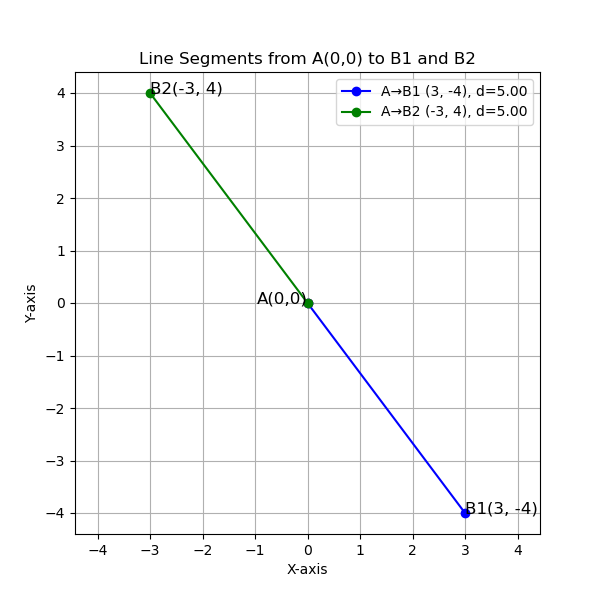
\includegraphics[width=\columnwidth, height=0.8\textheight, keepaspectratio]{figs/distance.png}     
\end{frame}

\begin{frame}[fragile]
    \frametitle{Python Code}
    \begin{lstlisting}
import numpy as np
import matplotlib.pyplot as plt

# Fixed point A
A = (0, 0)

# Two B points
B1 = (3, -4)
B2 = (-3, 4)

# Distances using numpy
d1 = np.sqrt((B1[0]-A[0])**2 + (B1[1]-A[1])**2)
d2 = np.sqrt((B2[0]-A[0])**2 + (B2[1]-A[1])**2)




\end{lstlisting}
\end{frame}

\begin{frame}[fragile]
    \frametitle{Python Code }
    \begin{lstlisting}
# Plot line segments A->B1 and A->B2
plt.figure(figsize=(6,6))

# Line A->B1
plt.plot([A[0], B1[0]], [A[1], B1[1]], 'b-o', label=f"A→B1 {B1}, d={d1:.2f}")
plt.text(B1[0], B1[1], f"B1{B1}", fontsize=12, ha='left')

# Line A->B2
plt.plot([A[0], B2[0]], [A[1], B2[1]], 'g-o', label=f"A→B2 {B2}, d={d2:.2f}")
plt.text(B2[0], B2[1], f"B2{B2}", fontsize=12, ha='left')


\end{lstlisting}
\end{frame}

\begin{frame}[fragile]
    \frametitle{Python Code }
    \begin{lstlisting}
# Mark A
plt.scatter(A[0], A[1], color='red')
plt.text(A[0], A[1], "A(0,0)", fontsize=12, ha='right')

# Labels & styling
plt.xlabel("X-axis")
plt.ylabel("Y-axis")
plt.title("Line Segments from A(0,0) to B1 and B2")
plt.legend()
plt.grid(True)
plt.axis("equal")
plt.savefig('figs/distance2.png')
9 subprocess.run(shlex.split("termux-open figs/distance2.png")

\end{lstlisting}
\end{frame}




\begin{frame}{Plot-Using only Python}
    \centering
    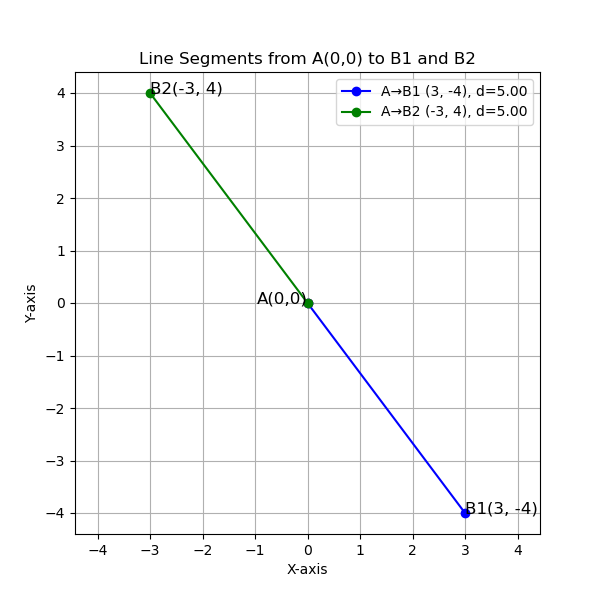
\includegraphics[width=\columnwidth, height=0.8\textheight, keepaspectratio]{figs/distance2.png}     
\end{frame}


\end{document}